\documentclass[qualitaetssicherung.tex]{subfiles}

\begin{document}
\section*{Vorwort}
Um die Testresultate auch später reproduzieren zu können, lohnt es sich die verwendete Umgebung zu dokumentieren.
\section{Entwicklungsumgebung}
	\begin{itemize}
		\item IDE: JetBrains WebStorm (11.0)
	\end{itemize}
\section{Ausführungsumgebung}
	\subsection{Server}
		\begin{itemize}
			\item Betriebssystem: Raspbian (4.1)
			\item HTTP Server: Node.js (5.7.0)
		\end{itemize}
	\subsection{Client}
		\begin{itemize}
			\item Webbrowser: Chrome (44.0) oder Firefox (42.0)
		\end{itemize}
\section{Werkzeuge fürs Testen}\label{werkzeuge}

\begin{itemize}
	
	\item

	Jasmine\newline	
	Um unsere Testfälle einfach und automatisiert durchlaufen lassen zu können, haben wir uns entschlossen eine bekannte Javascript-Testumgebung zu verwenden, die Jasmine heißt. Man schreibt die Testfälle in Typescript und danach führt man Jasmine aus: man soll in einer HTML Datei die Javascript Dateien von Jasmine, die Testdateien und die zu testende Dateien referenzieren. Wenn man die HTML Datei öffnet, werden die Tests durchgeführt und die Resultate automatisch angezeigt (Abb. ~\ref{jasmine_example}).
	
	\item
	Karma\newline
	Damit wir wissen, welche Code-Zeilen wir schon überprüft haben ist es von Vorteil ein Werkzeug zu haben, das uns die Codeabdeckung anzeigt (Abb. ~\ref{karma_example_1}) und uns beim Schreiben von Testfällen unterstützt (Abb. ~\ref{karma_example_2}). Als Tool zur Messung der Codeabdeckung haben wir Karma (verwendet intern Istanbul) ausgewählt.\newline

	\begin{figure}[H]
		\centering
    \textbf{Jasmine}\par\medskip
    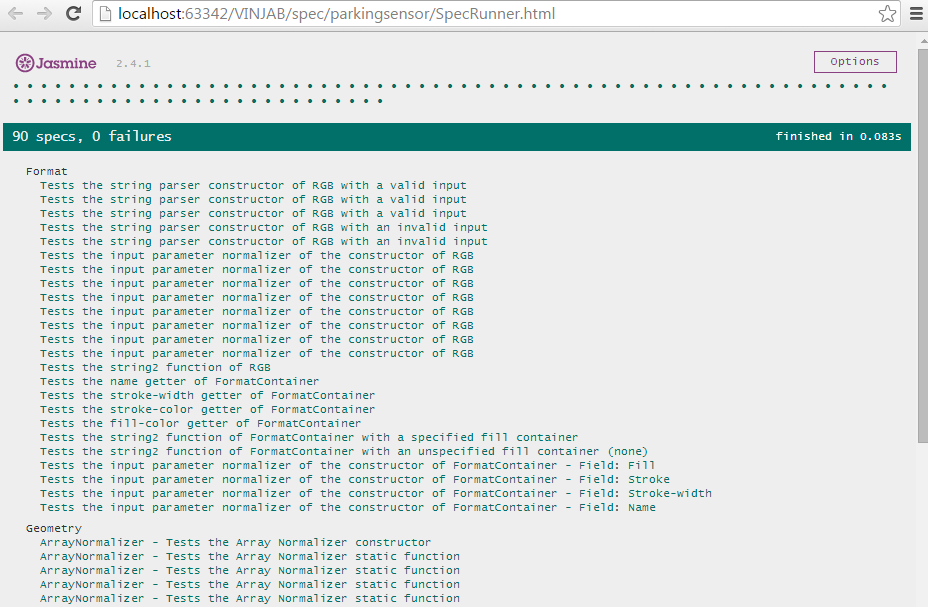
\includegraphics[width=0.8\textwidth]{Images/jasmine-example.png}
    \caption{So werden die Testresultate in Chrome dargestellt}
		\label{jasmine_example}
	\end{figure}
	
	\begin{figure}[H]
		\centering
    \textbf{Karma-Übersicht}\par\medskip
    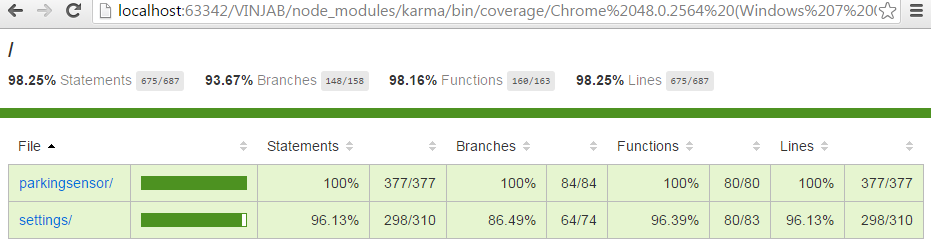
\includegraphics[width=0.8\textwidth]{Images/karma-example-1.png}
    \caption{Codeabdeckung bei den einzelnen Modulen}
		\label{karma_example_1}
	\end{figure}
	
	\begin{figure}[H]
		\centering
    \textbf{Karma-Abdeckung}\par\medskip
    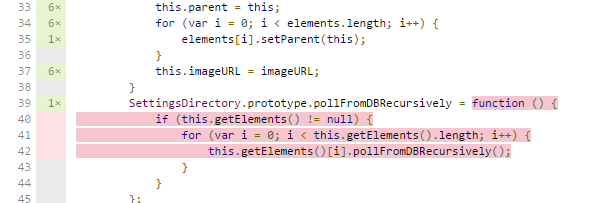
\includegraphics[width=0.8\textwidth]{Images/karma-example-2.png}
    \caption{Die nicht abgedeckte Codezeilen werden rot markiert}
		\label{karma_example_2}
	\end{figure}
	

\end{itemize}
		
\end{document}